% =============================================================================
% main.tex — Bachelor Thesis Template (ZHAW / IMS)
% Document class: KOMA-Script scrreprt (chapters as top level)
% =============================================================================
\documentclass[a4paper, 11pt, bibliography=totoc, listof=totoc]{scrreprt}

% --- Language -----------------------------------------------------------------
\usepackage[english]{babel}
% NOTE: csquotes and inputenc are loaded inside bathesis.sty — do NOT load here

% --- Thesis style (KOMA-Script based) ----------------------------------------
\usepackage{bastyl}

% --- Bibliography -------------------------------------------------------------
\usepackage[
  backend  = biber,
  style    = numeric,
  sorting  = none,
]{biblatex}
\addbibresource{references.bib}    % rename to your .bib file

% --- PDF inclusion (title page) -----------------------------------------------
\usepackage{pdfpages}

% --- Temporary: placeholder text (remove when writing real content) -----------
\usepackage{lipsum}

% --- Glossary / Acronym / Symbol definitions ----------------------------------
% =============================================================================
% glossary.tex — Central definitions for acronyms, symbols, and glossary terms
%
% Usage in text:
%   \gls{fpv}           → first use: "First-Person View (FPV)", then "FPV"
%   \gls{sym:omega}     → ω  (and it appears in the nomenclature list)
%   \gls{gl:propwash}   → propwash (and it appears in the glossary)
%
%   \glspl{fpv}         → plural form
%   \Gls{fpv}           → capitalized first letter
%   \acrfull{fpv}       → force full form: "First-Person View (FPV)"
%   \acrshort{fpv}      → force short form: "FPV"
%
% Build chain: pdflatex → makeglossaries → pdflatex → pdflatex
%   (latexmk handles this automatically)
% =============================================================================

% -----------------------------------------------------------------------------
% Acronyms
% -----------------------------------------------------------------------------
\newacronym{fpv}{FPV}{First-Person View}
\newacronym{pid}{PID}{Proportional-Integral-Derivative}
\newacronym{fft}{FFT}{Fast Fourier Transform}
\newacronym{rpm}{RPM}{Revolutions Per Minute}
\newacronym{esc}{ESC}{Electronic Speed Controller}
\newacronym{imu}{IMU}{Inertial Measurement Unit}
\newacronym{snr}{SNR}{Signal-to-Noise Ratio}
\newacronym{frf}{FRF}{Frequency Response Function}
\newacronym{mimo}{MIMO}{Multi-Input Multi-Output}
\newacronym{siso}{SISO}{Single-Input Single-Output}
\newacronym{cli}{CLI}{Command Line Interface}
\newacronym{csv}{CSV}{Comma-Separated Values}
\newacronym{oop}{OOP}{Object-Oriented Programming}
% Add more as needed...

% -----------------------------------------------------------------------------
% Symbols / Nomenclature
% -----------------------------------------------------------------------------
% \glssymbol{sym:omega} prints the symbol;  \gls{sym:omega} prints description.
% The 'sort' key controls alphabetical ordering in the list.

\newglossaryentry{sym:omega}{
  type        = symbols,
  name        = {\ensuremath{\omega}},
  description = {Angular frequency},
  sort        = {omega},
}

\newglossaryentry{sym:omegan}{
  type        = symbols,
  name        = {\ensuremath{\omega_n}},
  description = {Natural frequency},
  sort        = {omega n},
}

\newglossaryentry{sym:s}{
  type        = symbols,
  name        = {\ensuremath{s}},
  description = {Laplace variable},
  sort        = {s},
}

\newglossaryentry{sym:Kp}{
  type        = symbols,
  name        = {\ensuremath{K_p}},
  description = {Proportional gain},
  sort        = {Kp},
}

\newglossaryentry{sym:Ki}{
  type        = symbols,
  name        = {\ensuremath{K_i}},
  description = {Integral gain},
  sort        = {Ki},
}

\newglossaryentry{sym:Kd}{
  type        = symbols,
  name        = {\ensuremath{K_d}},
  description = {Derivative gain},
  sort        = {Kd},
}

\newglossaryentry{sym:P}{
  type        = symbols,
  name        = {\ensuremath{P(\omega)}},
  description = {Plant transfer function},
  sort        = {P},
}

\newglossaryentry{sym:C}{
  type        = symbols,
  name        = {\ensuremath{C(\omega)}},
  description = {Controller transfer function},
  sort        = {C},
}

\newglossaryentry{sym:S}{
  type        = symbols,
  name        = {\ensuremath{S(\omega)}},
  description = {Sensitivity function},
  sort        = {S},
}

\newglossaryentry{sym:T}{
  type        = symbols,
  name        = {\ensuremath{T(\omega)}},
  description = {Complementary sensitivity function},
  sort        = {T},
}
% Add more symbols as needed...

% -----------------------------------------------------------------------------
% Glossary Terms (optional — remove section if not using)
% -----------------------------------------------------------------------------
\newglossaryentry{gl:propwash}{
  name        = {propwash},
  description = {Turbulent airflow generated by the propellers that can
                 destabilize the drone when descending through its own wake},
}

\newglossaryentry{gl:blackbox}{
  name        = {Blackbox},
  description = {Betaflight's onboard data logging system that records
                 high-resolution flight data to a microSD card or flash memory},
}

\newglossaryentry{gl:chirp}{
  name        = {chirp signal},
  description = {A sinusoidal signal whose instantaneous frequency sweeps
                 continuously across a defined range, used for broadband
                 system excitation},
}
% Add more as needed...

\makeglossaries

% =============================================================================
% Thesis Metadata
% =============================================================================
\renewcommand{\thesistitle}{Betaflight -- Offline Controller Tuning}
\renewcommand{\thesissubtitle}{%
  Data-Driven Tuning of Rate and Altitude Controllers for FPV Drones%
}
\renewcommand{\thesisauthors}{Yuri Bianchi, Dario Jurietti and Janick Dort}
\renewcommand{\thesisdate}{\today}
\renewcommand{\thesisheader}{Betaflight - Offline Controller Tuning}
\renewcommand{\thesisfooter}{ZHAW / IMS}
% \renewcommand{\thesislogo}{imslogo.pdf}  % uncomment when logo file exists

% PDF metadata
\hypersetup{
  pdftitle    = {Betaflight -- Offline Controller Tuning},
  pdfauthor   = {Yuri Bianchi, Dario Jurietti, Janick Dort},
  pdfsubject  = {Bachelor Thesis, ZHAW School of Engineering},
  pdfkeywords = {Betaflight, PID tuning, system identification, FPV, chirp},
}

% =============================================================================
\begin{document}
% =============================================================================

% *****************************************************************************
%   FRONT MATTER
% *****************************************************************************
\frontmatter

% --- Title page ---------------------------------------------------------------
% Option A: External PDF (uncomment when Titelblatt.pdf exists)
% \begin{titlepage}
%   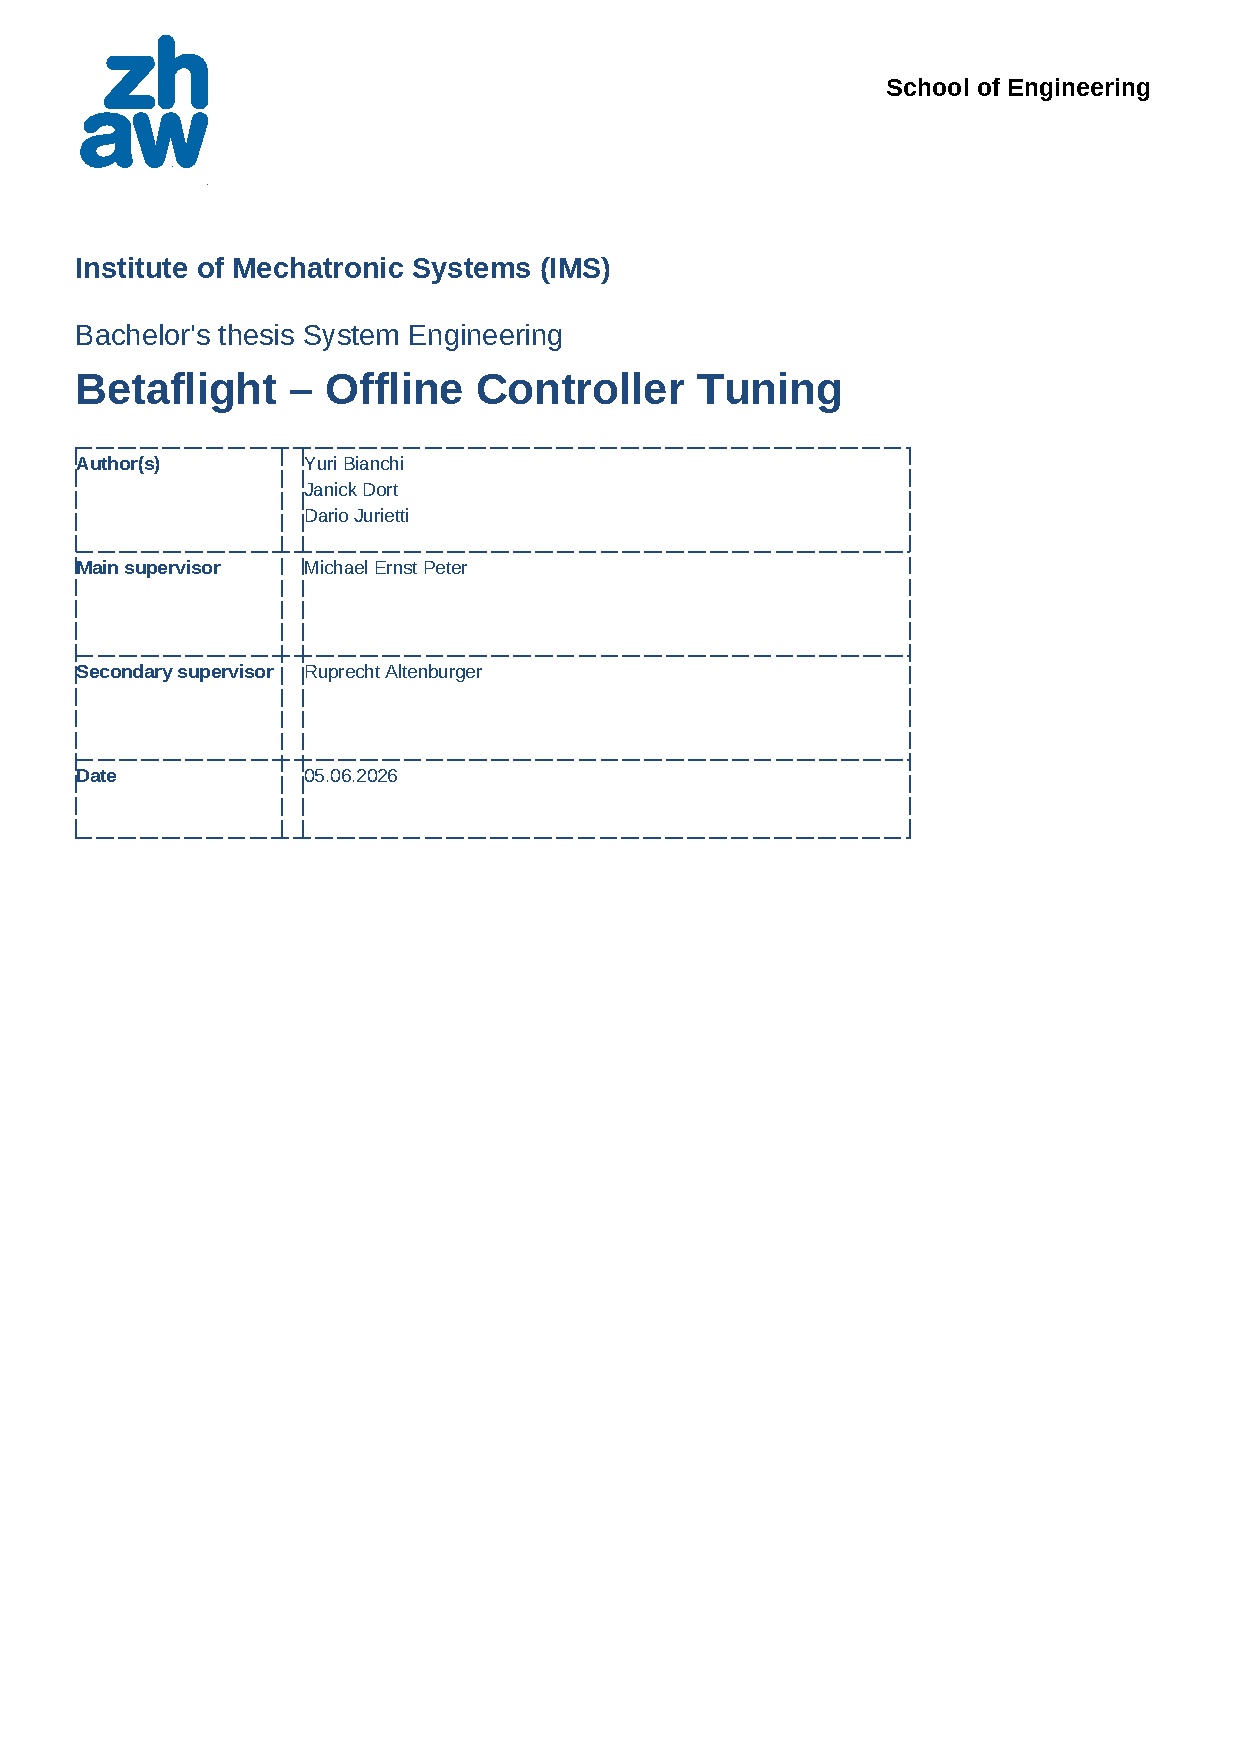
\includepdf[pages=1]{pdf/Titelblatt.pdf}
% \end{titlepage}

% Option B: Auto-generated fallback title page
\makethesistitle

% --- Declaration of Originality -----------------------------------------------
\makedeclaration{Winterthur}{\today}

% --- Abstract (German + English) ----------------------------------------------
\chapter*{Zusammenfassung}
\addcontentsline{toc}{chapter}{Zusammenfassung}

\lipsum[1] % placeholder — replace with German abstract

\chapter*{Abstract}
\addcontentsline{toc}{chapter}{Abstract}

\lipsum[2] % placeholder — replace with English abstract

% --- Table of Contents --------------------------------------------------------
\tableofcontents

% --- List of Figures ----------------------------------------------------------
\listoffigures

% --- List of Tables -----------------------------------------------------------
\listoftables

% --- Acronyms -----------------------------------------------------------------
\printglossary[type=\acronymtype, title={List of Acronyms}]

% --- Nomenclature (Symbols) ---------------------------------------------------
\printglossary[type=symbols, title={Nomenclature}]

% --- Glossary (optional — uncomment if using glossary terms) ------------------
% \printglossary[title={Glossary}]


% --- Preface / Acknowledgements -----------------------------------------------
\chapter*{Preface}
\addcontentsline{toc}{chapter}{Preface}

This thesis was carried out during the spring semester 2026 at the Institute of
Mechatronic Systems~(IMS) at the ZHAW School of Engineering. It continues the
work started in the preceding project thesis conducted in the fall semester 2025.

We would like to thank our supervisor, Michael Peter, for\ldots


\newpage
% *****************************************************************************
%   MAIN MATTER
% *****************************************************************************
\mainmatter


% =============================================================================
\chapter{Introduction}
\label{ch:introduction}

First-Person-View (FPV) racing drones require precise and responsive control to achieve stable
flight behaviour, suppress disturbances such as propeller wash, and maintain agility during rapid
manoeuvres. The flight performance strongly depends on the tuning of the flight controller’s
feedback loops. In particular, the parameters of the angular rate controller determine how
quickly and accurately the drone reacts to pilot inputs and external disturbances.

In practice, controller tuning is still often performed manually through iterative trial-and-error
procedures. This requires extensive flight testing and considerable piloting experience, making
the process time-consuming and difficult to reproduce. Although modern flight controller
firmware such as Betaflight provides extensive configuration options and detailed flight data
logging, systematic tuning remains a challenge.

One commonly used tool for offline tuning is the PID-Toolbox. In this approach, flight logs
are recorded during normal flights and later analysed to derive suitable controller parameters.
However, the system excitation depends entirely on the pilot’s inputs and the natural flight
behaviour of the drone. As a result, not all relevant frequency ranges are sufficiently excited,
which can limit the quality of the measurements.

In the approach proposed in this thesis, a chirp excitation signal is injected directly into
the control loop. This allows the system to be excited over a wide range of frequencies
in a controlled and systematic way, resulting in higher-quality measurements for system
identification and controller tuning.

A previous project introduced a proof-of-concept approach for offline tuning of angular rate
controllers based on recorded flight data. In the preceding project thesis, this concept was
restructured and modularised and now serves as the foundation for the present work.

The objective of this bachelor thesis is to further refine and extend this approach into an
offline tuning framework for multiple control loops used in Betaflight-based flight controllers.
In addition to the existing angular rate controller tuner, the framework will be extended with
code modules for tuning the angle controller, the altitude hold controller, and the position
controller. This extends the tuning framework beyond the inner rate control loop and enables
the analysis and tuning of higher-level control layers.

The framework will be implemented primarily in MATLAB and Python and will provide tools
for analysing flight logs, estimating system dynamics, and generating controller parameters
without requiring repeated flight tests. The software will be developed as an open-source
library with accompanying documentation for the FPV community.

By providing a structured, data-driven approach to controller tuning, this project aims to
simplify the tuning process and improve flight performance.

\newpage
% =============================================================================

\section{Initial situation}
\label{sec:IniSituation}

\section{Task and Objective}
\label{sec:TaskObjective}

\newpage

% =============================================================================
\chapter{Theoretical Foundations}
\label{ch:theory}

In this chapter, the theoretical background of the approach used for tuning the different control loops of the flight controller is introduced. Since the fundamental working principle is identical for all loops, the general concepts are explained here before addressing the individual loops in the methodology section.

To support the theoretical concepts, a simplified simulation model is introduced. The simulation is gradually developed throughout this chapter, allowing the reader to follow the modelling process step by step and to better understand the behaviour of the control system. This approach illustrates the influence of the controller parameters and provides an intuitive understanding of the tuning process.

The detailed application of these principles to the different control loops implemented in Betaflight is discussed in the following chapter.

\section{Chirp Signal}

\subsection{Mathematical Definition}

The instantaneous value of the chirp signal is defined as

\[
x(t) = \sin(\text{arg}(t)),
\]

where the phase argument

\[
\text{arg}(t) = 2\pi \int_0^t f(\tau)\,d\tau
\]

represents the instantaneous phase of the signal. In practical implementations such as
\textbf{Betaflight}, the phase is wrapped once it reaches $2\pi$. This keeps the numerical
values bounded and produces the sawtooth-shaped \texttt{sinarg} signal that is often
observed in practice.

The behaviour of the chirp signal is determined by several parameters that define the
frequency sweep:

\begin{itemize}
\item $f_0$ -- starting frequency of the chirp signal (in the simulation $1\,\text{Hz}$)
\item $f_1$ -- final frequency of the chirp signal (in the simulation $600\,\text{Hz}$)
\item $T$ -- total duration of the frequency sweep (in the simulation $20\,\text{s}$)
\item $f_s$ -- sampling frequency used in the discrete-time simulation (in the simulation $2000\,\text{Hz}$)
\end{itemize}

The parameters used in the simulation are chosen to be close to the typical operating range
of the real system.

\subsection{Common Frequency Profiles}

\textbf{Linear chirp:}

For a linear chirp, the instantaneous frequency increases linearly over time. 
The slope of the frequency sweep is defined as

\[
k = \frac{f_1-f_0}{T}.
\]

The instantaneous frequency is therefore given by

\[
f(t) = f_0 + k t,
\]

and the corresponding phase trajectory results from integrating the frequency over time

\[
\text{arg}(t) = 2\pi\left(f_0 t + \tfrac{1}{2}k t^2\right).
\]

Figure~\ref{fig:linear_chirp} illustrates the resulting chirp signal, the instantaneous
frequency $f(t)$, and the corresponding phase trajectory $\text{arg}(t)$ for the
simulation parameters introduced in the previous section.

\begin{figure}[h]
\centering

\includegraphics[width=1.0\textwidth]{linear_chirp.png}
\caption{Linear chirp signal used for the simulation.}
\label{fig:linear_chirp}
\end{figure}

The apparent gaps visible in the chirp signal and in the wrapped phase are caused by the finite sampling time of the simulation and the limited resolution of the plotted data, rather than by discontinuities in the signal itself.

\textbf{Exponential chirp (as used in Betaflight):}

For an exponential chirp, the instantaneous frequency increases exponentially
from the starting frequency $f_0$ to the final frequency $f_1$ over the time
interval $T$. The instantaneous frequency is defined as

\[
f(t) = f_0 \left(\frac{f_1}{f_0}\right)^{t/T}.
\]

The corresponding phase trajectory results from integrating the frequency over time

\[
\text{arg}(t) =
\frac{2\pi T f_0}{\ln(f_1/f_0)}
\left[
\left(\frac{f_1}{f_0}\right)^{t/T}-1
\right].
\]

These expressions define the phase trajectory $\text{arg}(t)$ used in the simulations
and in the \texttt{apply\_rotfiltfilt} method for time-dependent frequency shifting
of chirp signals. The resulting exponential chirp signal, the instantaneous
frequency, and the phase trajectory are illustrated in Figure~\ref{fig:exponential_chirp}.

\begin{figure}[h]
\centering

\includegraphics[width=1.0\textwidth]{exponential_chirp.png}
\caption{Exponential chirp signal used for the simulation.}
\label{fig:exponential_chirp}
\end{figure}

The apparent gaps in the chirp signal and the wrapped phase result from the
discrete sampling time of the simulation and the limited resolution of the plot.

\subsection{Lag Filter for Chirp Input Shaping}

Before the chirp signal is injected into the control loop, it is conditioned by a filter to address the differentiating behavior of the controller effort at low frequencies. This differentiating characteristic causes rising gain at low frequencies, which would lead to excessive motor response at the start of the chirp sweep and potentially cause saturation, compromising the quality of system identification data. The filter reduces low-to-mid frequency components of the chirp signal before injection, such that the combined response produces approximately uniform excitation across the frequency range.

The filter is configured with a pole at 3 Hz and a zero at 30 Hz. This configuration corresponds to the transfer function
\begin{equation}
	H(s) = \frac{1 + s/\omega_z}{1 + s/\omega_p}
\end{equation}
where $\omega_z = 2\pi \cdot 30$ rad/s and $\omega_p = 2\pi \cdot 3$ rad/s represent the zero and pole frequencies respectively. The pole introduces the lag component by creating magnitude reduction at frequencies above its cutoff frequency. The zero limits this reduction by introducing magnitude amplification at frequencies above its cutoff frequency. However, since the pole frequency is lower than the zero frequency, the pole's contribution dominates throughout the primary control bandwidth, resulting in a net lag filter. It is important to note that in the Betaflight implementation, the pole frequency ($\omega_p$) must not be set higher than the zero frequency ($\omega_z$), as this would create a lead filter that amplifies high frequencies and could potentially damage the motors.

For the simulation shown in Figure~\ref{fig:chirpleadlag}, the same parameter values introduced in the previous section were used ($f_0 = 1\,\text{Hz}$, $f_1 = 600\,\text{Hz}$, $T = 20\,\text{s}$, $f_s = 2000\,\text{Hz}$). The excitation signal is generated using the exponential chirp formulation described earlier.

\begin{figure}[H]
	\centering
	
\includegraphics[width=1.0\textwidth]{chirp_lag_filtert.png}
	\caption{Exponential chirp signal after conditioning with the lag filter used for chirp input shaping.}
	\label{fig:chirpleadlag}
\end{figure}

\section{Signal Processing}

To illustrate the influence of the applied signal processing steps, a simulation is used as a
reference. The simulated system approximates the dynamics of the drone attitude control
system and consists of an integrator, a first-order lag element, and a dead-time component.

The resulting transfer function is

\[
G(s)=G_1(s)\,G_2(s)\,G_t(s)
\]

with

\[
G_1(s)=\frac{\omega_1}{s}, \qquad
G_2(s)=\frac{1}{1+s/\omega_2}, \qquad
G_t(s)=e^{-s/\omega_t}.
\]

Thus, the overall transfer function becomes

\[
G(s)=\frac{\omega_1}{s}\cdot\frac{1}{1+s/\omega_2}\cdot e^{-s/\omega_t}.
\]

For the simulation, the parameters are chosen as

\[
\omega_1 = 16 \cdot 2\pi, \qquad
\omega_2 = 13 \cdot 2\pi, \qquad
\omega_t = 60 \cdot 2\pi.
\]

The structure of the simulation model is illustrated in Figure~\ref{fig:signal_processing_model}.
The chirp signal $u(t)$ is applied to the transfer function $G(s)$, resulting in the ideal
system output $\tilde{y}(t)$. To emulate realistic measurement conditions, additive
disturbance noise $d(t)$ is superimposed on the output, such that

\[
y(t) = \tilde{y}(t) + d(t).
\]

In the simulation, the disturbance is modelled as additive white Gaussian noise with a
standard deviation of $\sigma_d = 2\,\text{deg/s}$.

\begin{figure}[H]
	\centering
	
\includegraphics[width=0.8\textwidth]{signal_processing_block.png}
	\caption{Simulation model used for the signal processing analysis.}
	\label{fig:signal_processing_model}
\end{figure}

\subsubsection{Estimate Frequency Response}

For a meaningful estimation of the transfer function, the frequency response between the input and output signals is analyzed. 

In the frequency domain, the relation between the input and output of a linear time-invariant (LTI) system can be expressed as
\[
G(\omega) = \frac{Y(\omega)}{U(\omega)}.
\]

Here, \(U(\omega)\) and \(Y(\omega)\) denote the Fourier transforms of the input signal \(u(t)\) and the output signal \(y(t)\), respectively. This ratio describes how each frequency component of the input is scaled and phase-shifted by the system.

In practice, however, the measured output signal is affected by disturbances. The measured output can therefore be written as
\[
Y(\omega) = G(\omega)U(\omega) + D_y(\omega),
\]
where \(D_y(\omega)\) represents an additive disturbance at the output. If the transfer function were estimated directly by dividing \(Y(\omega)\) by \(U(\omega)\), the disturbance term would directly influence the result
\[
\frac{Y(\omega)}{U(\omega)} = G(\omega) + \frac{D_y(\omega)}{U(\omega)}.
\]

This expression shows that a direct estimation is highly sensitive to disturbances and measurement noise.

To mitigate this issue, it is advantageous to consider the relation between input and output in terms of spectral quantities. In a first step, spectral quantities can be formed directly from the Fourier transforms as
\[
S_{uu}(\omega) = |U(\omega)|^2, \qquad
S_{yu}(\omega) = Y(\omega)U^*(\omega).
\]

Based on these quantities, the transfer function can be expressed as
\[
G(\omega) = \frac{S_{yu}(\omega)}{S_{uu}(\omega)}.
\]

However, this formulation is equivalent to the direct division \(Y(\omega)/U(\omega)\) and therefore inherits the same sensitivity to disturbances. In particular, the disturbance term is fully contained in the cross-spectral quantity and directly propagates into the estimate, which may lead to significant deviations from the true system behavior.

A more robust formulation is obtained by defining the spectral densities in a statistical sense using expectation values. This reduces the influence of disturbances, provided that the noise is uncorrelated with the input signal. Since the expectation operator cannot be evaluated directly from finite measurement data, it must be approximated by averaging over multiple realizations or segments of the signals. In practice, this is achieved using spectral estimation techniques such as Welch’s method, which is introduced in the following section.

As shown in Fig.~\ref{fig:transfer_estimation}, the estimated transfer function closely follows the true system response in frequency regions where the signal-to-noise ratio is sufficiently high. In contrast, deviations occur in frequency ranges dominated by noise and disturbances, where the estimation becomes less reliable.

\begin{figure}[h]
    \centering
    
\includegraphics[width=\linewidth]{Bode_direct_meas.png}
    \caption{Bode plot of the true and estimated transfer function. Deviations between the curves occur in frequency regions dominated by noise and disturbances.}
    \label{fig:transfer_estimation}
\end{figure}

\subsection{Baseband Filtering via Frequency Rotation}

Measured signals are often contaminated by measurement noise and unwanted high-frequency
components. These disturbances can obscure the relevant information contained in the signal
and negatively affect subsequent analysis steps. To suppress these disturbances while
preserving the phase characteristics of the signal, a frequency-shifting filtering approach
is employed.

The method is based on shifting the frequency content of the signal to baseband, applying a
low-pass filter, and subsequently shifting the signal back to its original frequency range.
This allows the filtering operation to focus on a narrow frequency region around the signal
of interest.

The underlying principle can be understood using the Fourier shift theorem. Multiplication
of a signal $f(t)$ with a complex exponential results in a shift of its spectrum

$$
e^{i2\pi\xi_0 t} f(t)
\;\Longleftrightarrow\;
\hat{f}(\xi-\xi_0),
$$

which translates the spectrum by the frequency $\xi_0$.

In the present case, the signal of interest is a chirp signal with a continuously varying
instantaneous frequency. Therefore, the frequency shift must also be time-dependent. This is
achieved by introducing a complex phasor

$$
p(t)=e^{i\phi(t)},
$$

where $\phi(t)$ denotes the instantaneous phase of the chirp signal.

Multiplying the measured signal $x(t)$ with this phasor or its complex conjugate results in
a rotation of the signal spectrum toward baseband

$$
y_R(t)=x(t)p(t), \qquad
y_Q(t)=x(t)p^*(t).
$$

After this rotation step, the dominant signal component is centered around
$0\,\text{Hz}$, enabling efficient filtering using a low-pass filter.

\subsubsection{Baseband Filtering}

Once the signal has been shifted to baseband, a low-pass filter is applied to remove
high-frequency noise components. Since the useful signal is concentrated near zero
frequency, the filter can effectively suppress unwanted spectral components outside this
region.

To avoid phase distortion, forward-backward filtering is employed. This approach applies
the filter in both forward and reverse directions, resulting in zero-phase filtering.

The filtering operation yields the filtered baseband signals

$$
y_R(t) \rightarrow \tilde{y}_R(t), \qquad
y_Q(t) \rightarrow \tilde{y}_Q(t),
$$

which contain the desired signal components with reduced noise.

\subsubsection{Inverse Frequency Rotation}

After filtering in the baseband, the signal is shifted back to its original frequency
range. This is achieved by multiplying the filtered signals with the corresponding inverse
phasors and combining the results to obtain a real-valued signal

$$
x_f(t)
=
\mathrm{Re}
\left(
\frac{1}{2}
\left(
\tilde{y}_R(t)p^*(t)
+
\tilde{y}_Q(t)p(t)
\right)
\right).
$$

This operation reverses the initial frequency rotation and reconstructs a filtered version
of the original signal. The resulting signal $x_f(t)$ retains the phase characteristics of
the original signal while high-frequency noise components are effectively suppressed.

\subsubsection{Impact on Frequency Response Estimation}

The filtered signal is subsequently used for frequency response estimation. By reducing
noise prior to the spectral analysis, the signal-to-noise ratio is significantly improved,
leading to more reliable estimates of the transfer function.

The effect of the filtering approach is illustrated in Fig.~\ref{fig:bode_filtered}, where
the estimated transfer function based on the filtered signal is compared with the true
system response. A closer agreement between both curves indicates that the baseband
filtering effectively suppresses noise while preserving the relevant system dynamics.

\begin{figure}[h]
    \centering
    
\includegraphics[width=\linewidth]{bode_apply_rotfiltfilt.png}
    \caption{Bode plot of the true transfer function and the estimated transfer function
    based on the filtered signal. The filtering improves the signal-to-noise ratio and
    leads to a more accurate estimation.}
    \label{fig:bode_filtered}
\end{figure}
\subsection{Spectral Estimation using Welch’s Method}

To estimate the spectral densities $S_{yu}(\omega)$ and $S_{uu}(\omega)$ from finite data,
Welch’s method is employed. The spectral densities cannot be computed directly from the
expectation operator, since only finite time-domain measurements of the input and output
signals are available. Instead, these quantities must be estimated from the measured data.
In this work, Welch’s method is used to obtain reliable estimates of the power spectral
densities and cross-power spectral densities.

Let $u[n]$ and $y[n]$ denote the discrete-time input and output signals of length $N$.
In Welch’s method, the signals are divided into $K$ overlapping segments of length $L$.
Each segment is multiplied by a window function $w[n]$ in order to reduce spectral leakage.

The $k$-th windowed segment of the input signal can therefore be written as

$$
u_k[n] = u[n + kD]\, w[n], \qquad n = 0, \dots, L-1
$$

where $D$ denotes the shift between successive segments and determines the amount of
overlap between segments.

For each segment, the discrete Fourier transform (DFT) is computed

$$
U_k(\omega) = \sum_{n=0}^{L-1} u_k[n] e^{-j\omega n}
$$

and analogously for the output signal

$$
Y_k(\omega) = \sum_{n=0}^{L-1} y_k[n] e^{-j\omega n}.
$$

From these Fourier transforms, the periodogram estimate of the power spectral density
of the input signal for each segment is obtained as

$$
P_{uu,k}(\omega) = \frac{1}{L} |U_k(\omega)|^2.
$$

Similarly, the cross-periodogram between output and input is defined as

$$
P_{yu,k}(\omega) = \frac{1}{L} Y_k(\omega) U_k^*(\omega).
$$

Welch’s method reduces the variance of the spectral estimates by averaging the periodograms
over all segments. The resulting estimates of the power spectral density and the cross-power
spectral density are therefore given by

$$
S_{uu}(\omega) = \frac{1}{K} \sum_{k=1}^{K} P_{uu,k}(\omega)
$$

and

$$
S_{yu}(\omega) = \frac{1}{K} \sum_{k=1}^{K} P_{yu,k}(\omega).
$$

In addition, the power spectral density of the output signal is obtained as

$$
S_{yy}(\omega) = \frac{1}{K} \sum_{k=1}^{K} P_{yy,k}(\omega),
$$

with

$$
P_{yy,k}(\omega) = \frac{1}{L} |Y_k(\omega)|^2.
$$

These averaged spectral estimates are then used to compute the transfer function estimate

$$
G(\omega) = \frac{S_{yu}(\omega)}{S_{uu}(\omega)}.
$$

Furthermore, the coherence function can be defined as

$$
\gamma^2(\omega) = \frac{|S_{yu}(\omega)|^2}{S_{uu}(\omega)\, S_{yy}(\omega)}.
$$

The coherence takes values in the range $0 \leq \gamma^2(\omega) \leq 1$ and provides a
frequency-dependent measure of the linear relationship between input and output signals.
Values close to one indicate that the output is predominantly determined by the input,
whereas low values indicate that noise, disturbances, or nonlinear effects dominate the
measurement and reduce the reliability of the estimated transfer function.

\subsubsection{Estimated Transfer Function}

The estimated transfer function obtained from the averaged spectral quantities is compared
with the true system response in the frequency domain, as shown in Fig.~\ref{fig:transfer_estimation}.
A good agreement between both curves indicates that the spectral estimation provides a reliable
approximation of the underlying system dynamics. Deviations occur primarily in frequency regions
where the signal-to-noise ratio is low and the estimation becomes less accurate.

\begin{figure}[h]
    \centering
    
\includegraphics[width=\linewidth]{transferfunction_after_processing.png}
    \caption{Bode plot of the true and estimated transfer function. A good agreement between both curves indicates that the spectral estimation captures the system dynamics well.}
    \label{fig:transfer_estimation}
\end{figure}

In order to further assess the reliability of the estimated transfer function, the coherence
function is evaluated. Unlike the transfer function itself, the coherence provides a direct
measure of how strongly the output signal is linearly related to the input signal at each
frequency.

\subsubsection{Coherence Analysis}

The coherence corresponding to the estimated transfer function is shown in
Fig.~\ref{fig:coherence_estimation}. High coherence values indicate frequency regions in which
the output is strongly driven by the input signal and the transfer function estimate can be
considered reliable. In contrast, low coherence values indicate that noise, disturbances, or
nonlinear effects dominate the measurement, leading to increased uncertainty in the estimated
transfer function.

\begin{figure}[h]
    \centering
    
\includegraphics[width=\linewidth]{coherence_processing.png}
    \caption{Magnitude-squared coherence between input and output signals. Values close to one indicate a strong linear relationship and therefore a reliable transfer function estimate, whereas low values indicate reduced reliability due to noise and disturbances.}
    \label{fig:coherence_estimation}
\end{figure}



\section{Control Loop Calculations}

Although the flight controller consists of several nested control loops, their fundamental
structure is identical. Each loop follows the same basic feedback control principle and differs
mainly in the controlled variable and the chosen controller parameters. Therefore, instead of
analysing every loop individually from the beginning, a simplified model is used to explain the
underlying calculations and controller behaviour.

The simplified control structure used for the analysis consists of a controller $C$ and a plant $P$,
which describes the dynamic behaviour of the system being controlled.

Using this simplified model allows the general behaviour of the control loop and the
calculation of the controller terms to be explained in a clear and structured way.
The same principles are later applied to the individual control loops implemented
in the flight controller.

\subsection{Calculation of the Control Loop Components}

After the signal processing steps, the control loop components can be calculated.
As in the signal processing stage, the goal is to mitigate the influence of disturbances
and noise on the calculated control loop components. Therefore, only the input signal
of the control loop is used for the estimation.

The advantage of this approach is that

\begin{itemize}
\item the input signal is not affected by the back-calculation of the control loop and is therefore not influenced by disturbances or noise within the loop.
\item the input signal is not affected by filtering steps, since it is not measured but taken directly from the software. Consequently, it is not subject to measurement noise or disturbances.
\end{itemize}

This approach allows a more precise estimation of the transfer function. However,
it also means that the transfer functions of the individual control loop components
cannot be calculated directly. Instead, they must be obtained through mathematical
manipulations.

For example, consider a simplified control loop consisting of a controller $C(s)$
and a plant $P(s)$.

To calculate the transfer function of the controller $C(s)$, the following relation can be used

$$
C(s) =
\frac{Y(s)}{E(s)} =
\frac{Y(s)}{R(s) - Y(s)} =
\frac{Y(s)}{R(s)} \cdot
\frac{1}{1 - \frac{Y(s)}{R(s)}} =
\frac{G(s)}{1 - G(s)}.
$$

To calculate the transfer function of the plant $P(s)$, the following relation can be used

$$
P(s) =
\frac{Y(s)}{U(s)} =
\frac{Y(s)}{E(s)} \cdot
\frac{E(s)}{U(s)} =
C(s) \cdot \frac{1}{C(s)} = 1.
$$

\subsection{Closed-Loop Performance Metrics}

After determining the plant transfer function, the next step is to analyze the behaviour
of the overall system when a controller is applied. This is achieved by evaluating the
closed-loop transfer functions, which describe the system response, disturbance sensitivity,
disturbance rejection capability, and the required controller effort. These measures provide
valuable insights into the stability, robustness, and performance of the controlled system.

The closed-loop transfer function from the reference input to the output is given by

$$
G_{yr}(\omega) =
\frac{C(\omega)P(\omega)}
{1 + C(\omega)P(\omega)}.
$$

The sensitivity function, which describes how sensitive the system output is to
disturbances and model uncertainties, is defined as

$$
S(\omega) =
\frac{1}{1 + C(\omega)P(\omega)}.
$$

The compliance function, representing the system response to disturbances acting
on the plant, is given by

$$
SP(\omega) =
P(\omega)\,S(\omega).
$$

Finally, the controller effort describes the influence of the reference input on the
controller output and is defined as

$$
SC(\omega) =
C(\omega)\,S(\omega).
$$

\subsubsection{Step Response Analysis}

To be added.

% =============================================================================
\chapter{Methodology}
\label{ch:methodology}

In this chapter, the practical application of the theoretical concepts introduced in the previous chapter is described. The focus is on how these principles are implemented in the context of tuning the control loops of a Betaflight-based flight controller. The methodology is structured around the different control loops, starting with the angle controller, followed by the altitude hold controller and the position controller. For each control loop, the specific implementation details and tuning procedures are described.

\section{Angle Mode}

\subsection{Difference between Angle and Acro Mode}

The Betaflight software provides three main flight modes: Angle, Horizon, and Acro.

In Angle mode, the drone’s tilt angle is directly linked to the stick position. The maximum tilt is limited to a predefined value, preventing flips and making this mode particularly suitable for beginners.

In contrast, Acro mode provides full manual control. In this mode, stick inputs define an angular rate rather than a target angle, meaning the drone continues rotating as long as the stick remains deflected. This allows aggressive maneuvers such as flips and rolls but also requires greater pilot experience.

During the project thesis, an offline tuner for the angular rate controller was further developed to systematically optimize the rate control loop and improve Acro mode performance. The tuner was subsequently extended to also support Angle mode, enabling improved stability and responsiveness while maintaining intuitive handling for beginner pilots.

\subsection{Control Loops in Angle Mode}

In Angle mode, the angular rate controller is extended by an outer angle control loop, resulting in a cascaded control structure.

The stick input initially generates a rate setpoint. Unlike in Acro mode, this rate setpoint is then converted into a target angle. This target angle serves as the reference input for the inner angular rate controller.

The cascaded architecture separates attitude control from angular rate stabilization. While the outer loop ensures convergence toward the desired orientation, the inner loop provides fast dynamic stabilization by regulating the angular velocity. As a result, the system achieves improved disturbance rejection and more intuitive handling characteristics, since the pilot directly commands an angle rather than a rotational rate.

The Angle mode controller therefore consists of two cascaded loops:

\begin{itemize}
\item The outer angle loop, which computes the angle error
\item The inner angular rate loop, which computes the rate error
\end{itemize}

\begin{figure}[htbp]
    \centering
    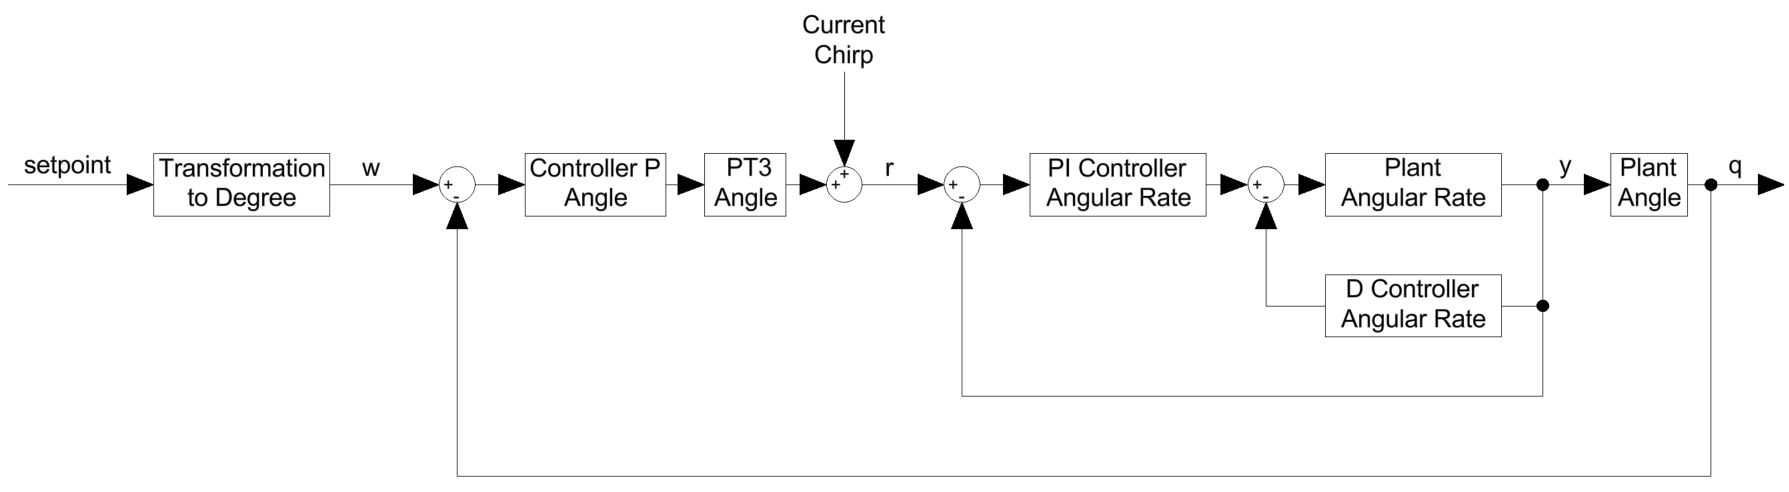
\includegraphics[width=1.0\textwidth]{Figures/Control_Loop_Angle.png}
    \caption{Cascaded control structure of the Betaflight Angle mode controller.}
    \label{fig:angle_mode_control_loop}
\end{figure}

The angle control loop consists of a proportional controller with an additional feedforward term. Within the offline tuning framework, however, only the proportional controller is optimized. The feedforward path is included in the control structure for completeness but was deliberately disabled during the tuning process.

\subsection{Derivation of the Target Angle}

The target angle is obtained by scaling the commanded angular rate with respect to the maximum achievable rate and the configured maximum tilt angle

\begin{equation}
\theta_{\text{target}} =
\theta_{\text{limit}}
\cdot
\frac{\omega_{\text{set}}}{\omega_{\text{max}}}
\tag{0.1}
\end{equation}

where

\begin{itemize}
\item $\theta_{\text{limit}}$ is the maximum allowed tilt angle (e.g., $60^\circ$),
\item $\omega_{\text{set}}$ is the commanded angular rate derived from the stick input,
\item $\omega_{\text{max}}$ is the maximum achievable angular rate determined by the rate configuration.
\end{itemize}

This relation ensures a proportional mapping between stick deflection and target angle.

For example,

\begin{equation}
\omega_{\text{set}} = \omega_{\text{max}}
\Rightarrow
\theta_{\text{target}} = \theta_{\text{limit}}
\tag{0.2}
\end{equation}

\begin{equation}
\omega_{\text{set}} = 0
\Rightarrow
\theta_{\text{target}} = 0
\tag{0.3}
\end{equation}

Thus, the stick position scales the target angle continuously within the range

\begin{equation}
-\theta_{\text{limit}}
\le
\theta_{\text{target}}
\le
+\theta_{\text{limit}}
\tag{0.4}
\end{equation}

\subsection{Chirp Signal for System Identification}

As already mentioned in the gyro control tuning section, a chirp signal is injected into the control loop.

If the chirp signal were added in the same way as for the gyro control tuning, it would not be
possible to directly calculate the transfer function of the complete system from the target
angle to the measured angle. The chirp signal would be added to the current setpoint and
therefore inside the closed control loop. Consequently, the system would have two inputs:
the stick input and the injected chirp signal.

This situation is illustrated in Figure~\ref{fig:angle_loop_original}, which shows the control
loop structure currently implemented in the Betaflight firmware.

\begin{figure}[htbp]
    \centering
    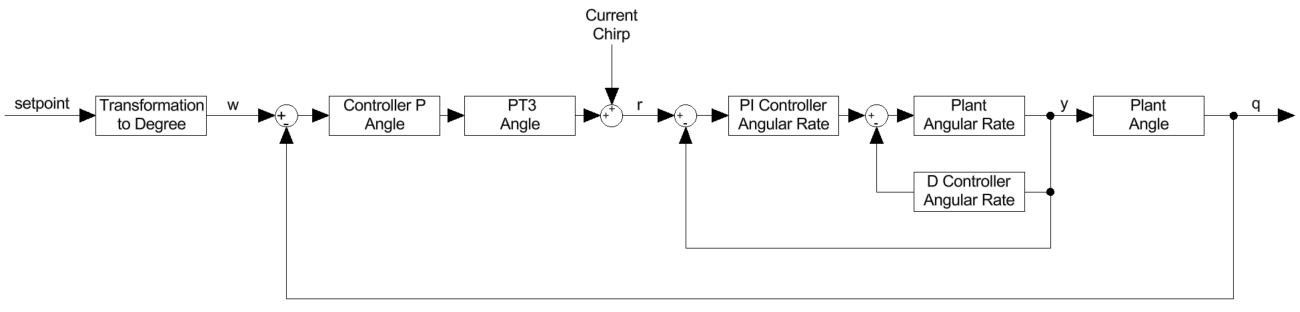
\includegraphics[width=1.0\textwidth]{Figures/Chirp_Control_Loop_Angle.png}
    \caption{Current control loop structure in Betaflight when the chirp signal is injected inside the closed loop.}
    \label{fig:angle_loop_original}
\end{figure}

To overcome this issue, a small modification in the firmware allows the chirp signal to be
added directly to the setpoint before it is converted into the target angle. Due to the
transformation from the setpoint to the target angle, the parameters of the chirp signal do
not need to be adjusted.

The modified control structure used for the offline tuning framework is illustrated in
Figure~\ref{fig:angle_loop_modified}. In this configuration, the chirp signal is injected
before the transformation from the rate setpoint to the target angle, allowing the transfer
function from the target angle to the measured angle to be estimated directly.

% TODO: Replace placeholder with final control loop diagram showing chirp injection before the angle conversion
%\begin{figure}[htbp]
   % \centering
    %\fbox{\rule{0pt}{6cm}\rule{0.9\textwidth}{0pt}}
    %\caption{Modified control loop structure with chirp injection before the target angle generation (to be created).}
    %\label{fig:angle_loop_modified}
%\end{figure}

Some older drones are only capable of flying in Acro mode and therefore do not support Angle
mode. In this case, the chirp signal can still be added to the setpoint. Since the angle control
loop and the transformation from the setpoint to the target angle are disabled in Acro mode,
the resulting control loop structure is identical to the one used for the gyro control tuning.

This approach allows the same chirp signal to be used for both modes. As a result, the
implementation is simplified and the tuning process becomes more straightforward, since the
same excitation signal can be applied without considering structural differences in the control
loop.

% *****************************************************************************
%   BACK MATTER
% *****************************************************************************
\backmatter

% --- References ---------------------------------------------------------------
\printbibliography[title={References}]

% --- Generative AI Declaration ------------------------------------------------
\chapter*{Declaration of Generative AI Use}
\addcontentsline{toc}{chapter}{Declaration of Generative AI Use}

The following generative AI systems were used during the preparation of this
thesis. Their use was limited to the functions described below. All generated
content was critically reviewed and verified by the authors.

% List AI tools as in your PA.

% --- Appendix -----------------------------------------------------------------
\appendix


% =============================================================================
\end{document}
